\chapter{Formal Concept Analysis}
\label{chapter:formal-concept-analysis}

\FCA (henceforth initialised to FCA) is an approach to reasoning about \textit{concepts} and corresponding \textit{conceptual structures} in terms of lattice theory. At the foundation of FCA is a philosophical viewpoint, tracing back to Aristotle, which describes concepts as a unit consisting of two parts, the dual between \textit{extension}: those things that exist as an instance of the concept; and \textit{intension}: the properties which give meaning to the concept \cite[p. 1]{WILLE1992493} \cite[p. 414]{DUQUENNE1999407}. As we will discuss in the following section, this perspective on concepts can be modelled quite elegantly by relations on sets of extensional and intensional elements. \index{extension} \index{intension}

\section{Basic Notions in Formal Concept Analysis}
\label{section:basic-notions}

The starting point in FCA is a structure called a \textit{formal context}, or simply a \textit{context}. A context represents the relational aspect between the extensional and intensional sets.
%
\begin{definition}
\label{definition:formal-context} \index{formal context}
  A \textit{formal context} $\GMI$ is a triple comprised of a set of objects $G$, a set of attributes $M$, and a binary relation $I \subseteq G \times M$ referred to as an `incidence' relation. For an object-attribute pair $(g,m) \in I$ we might say that \say{object $g$ \textit{has} the attribute $m$}.
\end{definition}
%
We regard the set $G$ of objects as being the extensional dimension of the context, while the set $M$ of attributes is intensional. Although, there is no strict requirement around what these sets are made up of, or that they be distinct---it is perfectly fine to have a context where $G$ and $M$ are the same sets.

It should be noted that, while the presence of an object–attribute pair $(g,m)$ in the incidence relation is interpreted as the object having the respective attribute, FCA is concerned with only \textit{positive} information, and so the absence of a pair in the relation is not usually interpreted to mean the object has the negation of the attribute.

When the cardinalities of $G$ and $M$ are small, contexts may be represented as a cross-table like \Cref{context:formal-context-group-structures} where each object is represented by a row in the table, each attribute by a column, and each element in the incidence relation is marked with an `$\times$' at the appropriate position \cite[pp. 17]{ganter1999formal}. Given a context is presented in this form, it is easy to identify all the attributes that a particular object satisfies: one need only scan across the respective row and note where the marks appear. The resulting set of attributes is called the \textit{object's intent}. The dual notion of an \textit{attribute extent} can be found by traversing down a column in the table.
\begin{example}
  \label{example:first-example-formal-context}
  Finite formal contexts of a reasonable size can be described entirely by a tabular representation. Each object corresponds to a row, and each attribute to a column.

  \begin{figure}[H]
    \centering
    \small
    \begin{cxt}
         \cxtName{\textbf{\texttt{Algebraic Structures}}}
      \att{\texttt{closure}} \att{\texttt{associativity}} \att{\texttt{identity}} \att{\texttt{divisibility}} \att{\texttt{commutativity}}
      \obj{x....}{\texttt{magma}}
      \obj{xx...}{\texttt{semigroup}}
      \obj{xxx..}{\texttt{monoid}}
      \obj{xxxx.}{\texttt{group}}
      \obj{xxxxx}{\texttt{abelian group}}
      \obj{x.xx.}{\texttt{loop}}
      \obj{x..x.}{\texttt{quasiagroup}}
      \obj{.xxx.}{\texttt{groupoid}}
      \obj{.xx..}{\texttt{category}}
      \obj{.x...}{\texttt{semicategory}}
    \end{cxt}
    \caption{A formal context showing necessary properties of group-like structures.}
    \label{context:formal-context-group-structures}
  \end{figure}
\end{example}

The efficacy of this approach obviously diminishes when we are interested in non-trivial contexts, or determining the intents or extents for sets of objects or attributes, respectively. We can instead formalise the procedure by defining \textit{derivation operators}:

\begin{definition}
     \label{definition:derivation-operators} \index{derivation operators}
  Given a formal context $\GMI$, the \textit{derivation operators} are two order-reversing maps $(\cdot)^\uparrow : 2^G \to 2^M$ and $(\cdot)^\downarrow : 2^M \to 2^G$ where the order is given by subset inclusion. Then, for any subsets $A \subseteq G$ and $B \subseteq M$,
  \begin{align*}
       A^\uparrow & \coloneqq \{m \in M \mid \forall g \in A, \; (g,m) \in I\} \\
       B^\downarrow & \coloneqq \{g \in G \mid \forall m \in B, \; (g,m) \in I\}
  \end{align*}
\end{definition}

It is common to denote either derivation operator with a prime and use the surrounding context to resolve ambiguity, so $A^\uparrow$ and $B^\downarrow$ would become $A'$ and $B'$, respectively. We avoid this notation as later on it will become increasingly challenging to avoid ambiguity while maintaining pleasing notation.

The derivation operators provide a clear way of describing, for a given set $A\subseteq G$ of objects, the set of attributes which every object in $A$ satisfies, denoted $A^\uparrow$. As an illustration, given the set of objects $\{\texttt{semigroup, monoid}\}$ from \Cref{context:formal-context-group-structures}, its derivation would be $\{\texttt{closure, associativity}\}$. It is quite easy to spot that this is just the intersection of the object intents of \texttt{semigroup} and \texttt{monoid}.

Of course, these two functions can be composed; and so, $A^{\uparrow \downarrow}$---which can rather cumbersomely be described as \say{the set of all objects which satisfy all the attributes satisfied by \texttt{semigroup} and \texttt{monoid}}---would yield the set $\{\texttt{semigroup, monoid, group, abelian group}\}$. In fact, this composition of derivation operators satisfies very specific properties, \index{closure operator}
\begin{align}
  & \text{(monotonicity)} & A \subseteq A_1 \textit{ implies } A^{\uparrow \downarrow} \subseteq A_1^{\uparrow \downarrow} \\
  & \text{(extensivity)}  & A \subseteq A^{\uparrow \downarrow} \\
  & \text{(idempotency)}  & A^{\uparrow \downarrow} = (A^{\uparrow \downarrow})^{\uparrow \downarrow}
\end{align}
for all $A, A_1 \subseteq G$. Thus, $(\cdot)^{\uparrow \downarrow}$ describes a closure operator on the powerset $2^G$ of objects. The dual notion holds for attributes, and $(\cdot)^{\downarrow \uparrow}$ describes a closure operator on $2^M$ \cite[pp. 18]{ganter1999formal}.

\begin{proposition}
  \label{proposition:properties-about-derivation-operators}
  Let $\GMI$ be a formal context with subsets $A_0, A_1, A_2 \subseteq G$ and $B_0, B_1, B_2 \subseteq M$ of attributes. Then,
  \vspace{-1em}
  \begin{center}
    \begin{minipage}[t]{0.48\textwidth}
      \begin{enumerate}
        \item $A_0 \subseteq A_1 \Rightarrow A_1^\uparrow \subseteq A_0^\uparrow$
        \item $A_0 \subseteq A_0^{\uparrow \downarrow}$
        \item $A_0^\uparrow = A_0^{\uparrow \downarrow \uparrow}$
      \end{enumerate}
    \end{minipage}%
    \hfill
    \begin{minipage}[t]{0.48\textwidth}
      \begin{enumerate}
        \item $B_0 \subseteq B_1 \Rightarrow B_1^\downarrow \subseteq B_0^\downarrow$
        \item $B_0 \subseteq B_0^{\downarrow \uparrow}$
        \item $B_0^\downarrow = B_0^{\downarrow \uparrow \downarrow}$
      \end{enumerate}
    \end{minipage}
  \end{center}
\end{proposition}

The first point in \Cref{proposition:properties-about-derivation-operators} describes the process where as the size of a set of objects grows, the number of attributes that all objects in the set satisfy is reduced, and vice versa.

Let us temporarily speak imprecisely and consider the fairly general concept of a `human'. The size of this concept's extension---those things which may be considered as instance of `human'---is quite large. Consider another concept, `optometrist'. The extension of this latter concept is, presumably, considerably smaller than the former (and, we can be reasonably sure it would constitute a strict subset). It is also quite clear that the intension---those properties we associate with optometrists---would be larger (a superset) than those associated with `human'.

We have just, quite informally, described what constitutes a \textit{Galois connection} between the sets $(2^G, \subseteq)$ and $(2^M, \subseteq)$ induced by the two derivation operators.

\begin{definition}
  \label{definition:galois-connection} \index{galois connection}
  Given two partially ordered sets $\mathbf{X}$ and $\mathbf{Y}$, an \textit{antitone Galois connection} is a pair of functions $f:\mathbf{X}\!\to\!\mathbf{Y}$ and $g:\mathbf{Y}\!\to\!\mathbf{X}$ such that $y \preceq_Y f(x)$ if and only if $x \preceq_X g(y)$ for all $x\in X$ and $y\in Y$.
\end{definition}

With the above relationship between sets of objets and attributes in mind, it is appropriate to introduce a \textit{formal concept}.

\begin{definition}
  \label{definition:formal-concept} \index{formal concept}
  A \textit{formal concept} of a formal context $\GMI$  is a pair $(A,B)$ of subsets $A \subseteq G$ and $B \subseteq M$ that satisfies $A^\uparrow = B$ and $B^\downarrow = A$. Then, we say that $A$ is the concept \textit{extent} and that $B$ is the \textit{intent}. We write $\BGMI$ to denote the set of all concepts of $\GMI$.
\end{definition}

We can prescribe a rather intuitive ordering over concepts induced by the \textit{subconcept–superconcept} relation. If $(A_0, B_0)$ and $(A_1, B_1)$ are two concepts in a context, then $(A_0, B_0)$ is a \textit{subconcept} of $(A_1, B_1)$ if and only if $A_0 \subseteq A_1$, equivalently if $B_1 \subseteq B_0$. Otherwise, $(A_0, B_0)$ is a \textit{superconcept} of $(A_1, B_1)$. We denote set of all concepts ordered in this way by $\CLGMI$, and call this set the \textit{concept lattice} of $\GMI$.

\subsection{Attribute Implications}
\label{subsection:attribute-implications}

In FCA, attribute implications represent dependencies that exist between attributes in a context. If $M$ is a non-empty set of attributes with $A, B \subseteq M$, then we denote an attribute implication over $M$ as $A \rightarrow B$.

\begin{definition}
     \label{definition:attribute-implication}
     Let $M$ be a non-empty set of attributes, then an \emph{attribute implication} over $M$ is a
\end{definition}


If we examine the context in \Cref{context:voting-records-small} it is apparent that every representative who voted in favour of the proposed crime bill also voted in favour of the immigration bill; we write this dependency as $\texttt{crime} \rightarrow \texttt{immigration}$.



\begin{figure}[H]
\centering
    \begin{cxt}
         \cxtName{\textbf{\texttt{Congressional Voting Records}}}
         \atr{\texttt{mx-missile}}
         \atr{\texttt{crime}}
         \atr{\texttt{immigration}}
         \atr{\texttt{satellite ban}}
         \atr{\texttt{education}}
         \atr{\texttt{republican}}
         \atr{\texttt{democrat}}
         \obj{.xx.xx.}{\texttt{Representative 1}}
         \obj{......x}{\texttt{Representative 4}}
         \obj{.x..xx.}{\texttt{Representative 9}}
         \obj{..x.x.x}{\texttt{Representative 17}}
    \end{cxt}
    \caption{A context describing a portion of congressional voting records for 1984}
    \label{context:voting-records-small}
\end{figure}

\clearpage

\begin{figure}[H]
  \centering
  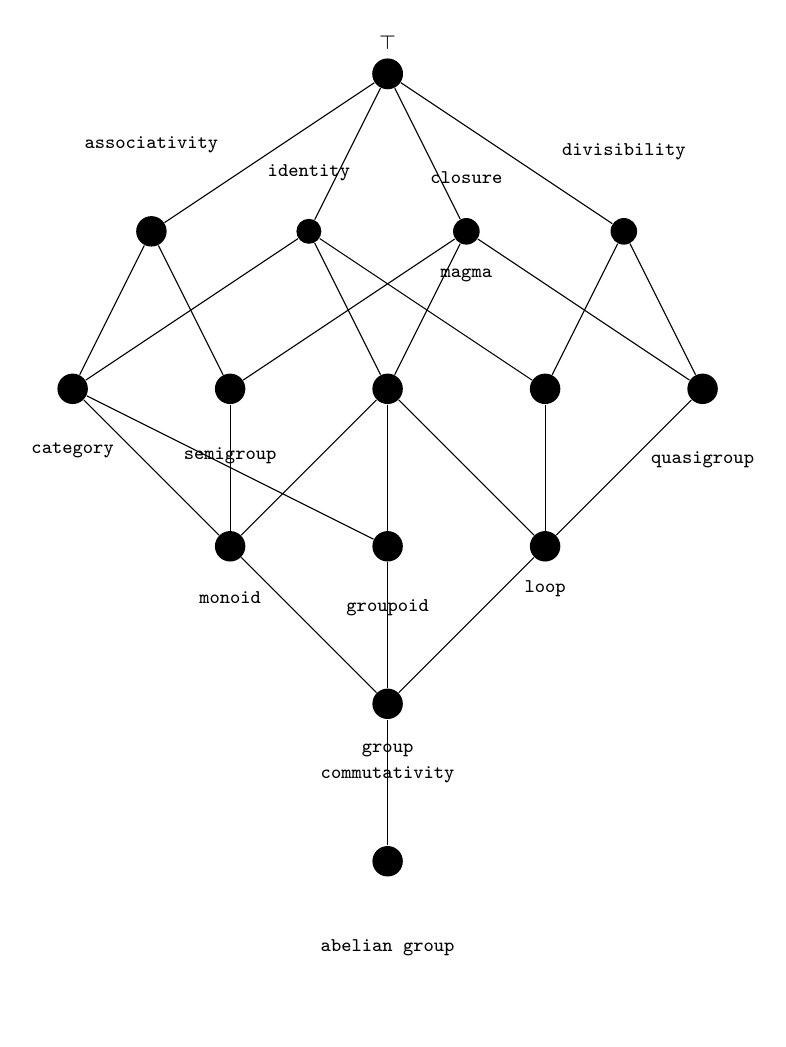
\begin{tikzpicture}[every node/.style={circle, fill=black, inner sep=1pt}]
    \node (a1) at (0,3) [label=above:{\scriptsize $\top$}] {w};
    % \node[draw=none, fill=none] at (0,3.5) {\tiny Top};

    \node (b1) at (-3,1) [label=above:{\scriptsize \texttt{associativity}}] {y};
    \draw (a1) -- (b1);

    \node (b2) at (-1,1) [label=above:{\scriptsize \texttt{identity}}] {z};
    \draw (a1) -- (b2);

    \node (b3) at (1,1) [label=above:{\scriptsize \texttt{closure}},label=below:{\scriptsize \texttt{magma}}] {x};
    \draw (a1) -- (b3);

    \node (b4) at (3,1) [label=above:{\scriptsize \texttt{divisibility}}] {x};
    \draw (a1) -- (b4);

    \node (c1) at (-4,-1) [label=below:{\scriptsize \texttt{category}}] {y};
    \draw (c1) -- (b1);
    \draw (c1) -- (b2);

    \node (c2) at (-2,-1) [label=below:{\scriptsize \texttt{semigroup}}] {y};
    \draw (c2) -- (b1);
    \draw (c2) -- (b3);

    \node (c3) at (0,-1) {y};
    \draw (c3) -- (b2);
    \draw (c3) -- (b3);

    \node (c4) at (2,-1) {y};
    \draw (c4) -- (b2);
    \draw (c4) -- (b4);

    \node (c5) at (4,-1) [label=below:{\scriptsize \texttt{quasigroup}}] {y};
    \draw (c5) -- (b3);
    \draw (c5) -- (b4);

    \node (d1) at (-2,-3) [label=below:{\scriptsize \texttt{monoid}}] {y};
    \draw (d1) -- (c1);
    \draw (d1) -- (c2);
    \draw (d1) -- (c3);

    \node (d2) at (0,-3) [label=below:{\scriptsize \texttt{groupoid}}] {y};
    \draw (d2) -- (c1);
    \draw (d2) -- (c3);

    \node (d3) at (2,-3) [label=below:{\scriptsize \texttt{loop}}] {y};
    \draw (d3) -- (c3);
    \draw (d3) -- (c4);
    \draw (d3) -- (c5);

    \node (e1) at (0,-5) [label=below:{\scriptsize \texttt{group}}] {y};
    \draw (e1) -- (d1);
    \draw (e1) -- (d2);
    \draw (e1) -- (d3);

    \node (f1) at (0,-7)[label=above:{\scriptsize \texttt{commutativity}},label=below:{\scriptsize \texttt{abelian group}}] {y};
    \draw (f1) -- (e1);
  \end{tikzpicture}
  \caption{The concept lattice associated with the formal context in \Cref{context:formal-context-group-structures}}
\end{figure}

\section{Contextual Attribute Logic}
\label{section:contextual-attribute-logic}

The logic that underlies FCA
\cite{ganter2025language, ganter1999contextual}
